\documentclass[a4paper,12pt,twoside,BCOR=10mm]{scrbook}

% Packages
\usepackage[utf8]{inputenc} % Updated by Ernir
\usepackage[icelandic]{babel} % Updated by Ernir
\usepackage[T1]{fontenc} % Updated by Ernir

\usepackage{graphicx}
\usepackage[intoc]{nomencl}
\usepackage{enumerate,color}
\usepackage{url}
\usepackage[pdfborder={0 0 0}]{hyperref}
\usepackage{appendix}
\usepackage{eso-pic}
\usepackage{amsmath, amssymb} % Inlined by Ernir
\usepackage[numbib,nottoc]{tocbibind} % Numbib option added by Ernir
\usepackage[sort&compress,authoryear]{natbib}
\usepackage{subcaption} % Obsolete subfigure package removed by Ernir
\usepackage[format=plain,labelformat=simple,labelsep=colon]{caption}
\usepackage{placeins}
\usepackage{tabularx}

%%% ADDITIONS BY ERNIR
\usepackage{textcomp} % To disable font warnings http://www.latex-community.org/forum/viewtopic.php?t=8608
\usepackage{scrhack} % To suppress KOMA warning http://tex.stackexchange.com/questions/51867/koma-warning-about-toc
\usepackage{booktabs}
\usepackage[newfloat]{minted}
\usepackage[rounded]{syntax}
\usepackage{auxhook}

\SetupFloatingEnvironment{listing}{name=Kóðalistun}
\SetupFloatingEnvironment{listing}{listname=Kóðalistunarskrá}

% Custom references
\newcounter{labelknownref}
\renewcommand*{\thelabelknownref}{\the\value{labelknownref}}
\makeatletter
\AddLineBeginAux{%
  \string\providecommand\string\LabelKnown[2]{}%
}
\newcommand*{\LabelKnown}[2]{%
  \expandafter\xdef\csname lkr@#2\endcsname{%
    \@ifundefined{r@#1}{0}{1}%
  }%
}

\newcommand*{\myref}[1]{%
  \begingroup
    \stepcounter{labelknownref}%
    \if@filesw
      \protected@write\@auxout{}{%
        \string\LabelKnown{#1}{\thelabelknownref}%
      }%
    \fi 
    \if\csname lkr@\thelabelknownref\endcsname 1%
      ($\leftarrow$\ref{#1})%
    \else
      \if\csname lkr@\thelabelknownref\endcsname 0%
        (\ref{#1}$\rightarrow$)%
      \else
        (\ref{#1})%
      \fi
    \fi
  \endgroup
}
\makeatother


% Syntax diagrams
\newenvironment{repnull}[0]{%
\begin{stack}
\\
\begin{rep}
}{%
\end{rep}
\end{stack}
}
\newenvironment{syntaxenv}[1]{%
\par\noindent\begin{minipage}{\linewidth}\vspace{0.5em}\begin{quote}\noindent%
\hspace*{-2em}\synt{#1}:\hfill\par%
\noindent%
\begin{minipage}{\linewidth}\begin{syntdiag}%
}{%
\end{syntdiag}\end{minipage}\end{quote}\end{minipage}%
}
%%% END ADDITIONS



% Configurations
\graphicspath{{figs/}}

\setlength{\parskip}{\baselineskip}
\setlength{\parindent}{0cm}
\raggedbottom

% Mun fallegri lausn
\setkomafont{captionlabel}{\itshape}
\setkomafont{caption}{\itshape}
\setkomafont{section}{\FloatBarrier\Large}
% \setcapwidth[l]{\textwidth} % Ernir: Kommentað út til að þagga niður í viðvörun um að þetta hafi verið hunsað
\setcapindent{1em}

%%%%%%%%%%% MODIFY THESE LINES ONLY %%%%%%%%%%%%%%%%%%%%%%%%%%%%%%%%%%%%%%%%%%%%%%%%%%%%%%%%%
\def\thesisyear{}       						% Year thesis submitted
\def\thesismonth{}						% Month thesis submitted
\def\thesisauthor{Eiríkur Ernir Þorsteinsson}					% Thesis authoreiningaraðferðinni
\def\thesistitle{Vefkennsla í notkun gagnasafna} 						% Title of thesis
\def\thesisshorttitle{Vefkennsla í notkun gagnasafna} 	% Title of thesis
\def\thesiscredits{40} 							% Credits awarded for the project
\def\thesissubject{Menntun framhaldsskólakennara}
\def\thesiskind{M.Sc.}							% Masters of PhD thesis
\def\thesiskindformal{Magister Scientiarum}				% Masters of PhD thesis
\def\thesisnroftutors{1}						% Number of tutors
\def\thesisschool{Verkfræði- og náttúruvísindasvið}			% School
\def\thesisfaculty{Iðnaðarverkfræði-, vélaverkfræði- og tölvunarfræðideild}							% Faculty
\def\thesisaddress{Hjarðarhaga 2-6}				% Office address
\def\thesispostalcode{107 Reykjavík}			% Office address
\def\thesistelephone{699-4392}						% Office telephone
\def\thesispublisher{-}						% Publisher
\def\thesistutors{Hjálmtýr Hafsteinsson}
\def\thesisrepresentative{XXNN3}					% Tutors name
\def\thesiscommittee{XXNN4 \\ XXNN5 }
\def\thesiskeywords{SQL, Exploratory Learning}			% Keywords
\def\thesisISBN{XX}           						% Thesis ISBN number
\def\thesisdedication{Dedication}
\def\thesisPrinting{Háskólaprent, Fálkagata 2, 107 Reykjavík}

% Function to add footer to frontpage
\newcommand\BackgroundPic{
\put(0,0){
\parbox[b][\paperheight]{\paperwidth}{
\vfill
\centering
\hspace*{-0.6cm}

\includegraphics[width=\paperwidth,height=\paperheight,
keepaspectratio]{foot}
}}
\setlength{\unitlength}{\paperwidth}
\begin{picture}(0,0)(0,-0.15)
\put(0,0){\color{white}\parbox{1\paperwidth}{\centering\bfseries\sffamily \Large \thesisfaculty \\
Háskóli Íslands\\
\thesisyear}}
\end{picture}
}

\begin{document}

\hypersetup{pageanchor=false}
\begin{titlepage}
\thispagestyle{empty}
\AddToShipoutPicture*{\BackgroundPic}
%
\begin{center}
\vspace*{1cm}

\includegraphics[width=43.6mm]{logotitle}\\
\vspace*{3.0cm}
\huge \sffamily \bfseries \thesistitle

\vspace*{5.5cm}
\normalfont \Large \sffamily \thesisauthor
\AddToShipoutPicture*{\BackgroundPic}
\vfill

\end{center}

\newpage 
\thispagestyle{empty} \mbox{}
\newpage
\vspace*{1.35cm}
\thispagestyle{empty}
\begin{center}

\Large \textbf{\sffamily{\MakeUppercase{\thesistitle}}} \\

\vspace*{1.7cm}
\sffamily{\thesisauthor} \\
\vspace*{1.8cm}
\normalsize \thesiscredits~ECTS thesis submitted in partial fulfillment of a \\
\textit{\thesiskindformal} degree in \thesissubject

\vspace*{1.0cm}
\large
\ifnum\thesisnroftutors >1 Advisors \\ \thesistutors \\ \vspace*{0.4cm}
\else Advisor \\ \thesistutors \\ \vspace*{1.04cm}
\fi
Faculty Representative \\
\thesisrepresentative

\vspace*{0.4cm}
M.Sc. committee \\
\thesiscommittee

\vfill
Faculty of \thesisfaculty \\
\thesisschool \\
University of Iceland \\
Reykjavik, \thesismonth~\thesisyear
\newpage
\end{center}
 \newpage
 \thispagestyle{empty}
 \mbox{} \vfill
 % \setcounter{page}{0} \renewcommand{\baselinestretch}{1.5}\normalsize
 \sffamily{\thesistitle} \\
 \sffamily{\thesisshorttitle} \\
 \thesiscredits ~ECTS thesis submitted in partial fulfillment of a \thesiskind~degree in \thesissubject
\\ \\
Copyright \textcopyright~\thesisyear~ \thesisauthor \\
All rights reserved \\


Faculty of \thesisfaculty \\
\thesisschool \\
University of Iceland \\
\thesisaddress \\
\thesispostalcode, Reykjavik \\
Iceland

Telephone: \thesistelephone \\ \\
\vspace*{\lineskip}

Bibliographic information: \\
\thesisauthor, \thesisyear, \thesistitle, \thesiskind~thesis, Faculty of \thesisfaculty, University of Iceland. \\

ISBN~\thesisISBN

Printing: \thesisPrinting \\
Reykjavik, Iceland, \thesismonth~\thesisyear \\
% \newpage
% \thispagestyle{empty} \mbox{}
% \vfill
% \begin{center}\textit{\thesisdedication}\end{center} \vspace*{5cm}
% \vfill 

\thispagestyle{empty}
\cleardoublepage
\end{titlepage}
\hypersetup{pageanchor=true}

% \dedication{\textit{Dedication} \small \\ Tileinkun má sleppa og skal þá fjarlægja blaðsíðuna. \\
% Tileinkun skal birtast á oddatölu blaðsíðu (hægri síðu).}
\pagenumbering{roman}

\setcounter{page}{5}
\section*{\huge Abstract}
Útdráttur á ensku sem er að hámarki 250 orð.
\vfill \vspace*{1cm}
\section*{\huge Útdráttur}
Hér kemur útdráttur á íslensku sem er að hámarki 250 orð. Reynið að koma útdráttum á eina blaðsíðu en ef tvær blaðsíður eru nauðsynlegar á seinni blaðsíða útdráttar að hefjast á oddatölusíðu (hægri síðu).
\vfill
\newpage

\tableofcontents
\listoffigures
\listoftables
\listoflistings

% \chapter*{Acknowledgments}
% \addcontentsline{toc}{chapter}{Acknowledgments}
% 
% Hjálmtýr Hafsteinsson
% 
% Hrefna Karítas Sigurjónsdóttir

\chapter{Inngangur}

\pagenumbering{arabic}
\setcounter{page}{1}

\section{Forsaga verkefnisins}
Sumarið 2014 skrifaði höfundur stutta kennslubók, til stuðnings við kennslu í fyrstu áföngum Tækniskólans í Reykjavík í notkun gagnasafna. Lagst var í skrifin eftir að ljóst var að nálgun nýlegra íslenskra bóka um gagnasafnsfræði\cite{sigurdur2003, jon2008} hentaði illa fyrir 16 til 17 ára nemendur.

Þarfir áfanganna í Tækniskólanum eins og þeir voru kenndir á þeim tíma voru í forgrunni við skrif bókarinnar. Farið var hægt yfir grundvallaratriði fyrirspurna og annarra mikið notaðra atriða í MySQL gagnagrunnskerfinu.

Kennslubókin var, með styrk frá Þróunarsjóði námsgagna, gefin út rafrænt sem PDF-skjal. Bókin var og er öllum aðgengileg á Github-síðu höfundar\footnote{\url{https://github.com/Ernir/sql-bok-ts}}. 

Bókinni var vel tekið af þeim kennurum Tækniskólans sem sáu um kennslu í notkun gagnasafna. Engu að síður varð fljótt ljóst að efninu mætti betur koma til skila með öðrum hætti - í gegnum vafrann.
\section{Önnur kennslutól}
Hugmyndin um að nýta vefinn og tölvuforrit til kennslu í notkun gagnasafna er ekki ný af nálinni. Auðvelt er að finna umfjöllun um eldri kennsluforrit sem upprunin eru í akademísku umhverfi. Auk þess hefur verið gríðarmikil gróska í gerð ýmissa veftóla til SQL-kennslu sem búin hafa verið til utan háskólaumhverfis. Verður nokkrum þeirra lýst hér að neðan.

\subsection{Akademísk SQL-kennslutól}
SQL-Tutor \cite{mitrovic1998} er kerfi komið til ára sinna, en þróun á því hófst árið 1996. Kerfið er, ætlað til að uppfylla hlutverk leiðbeinanda þegar nemandi vinnur að því að semja fyrirspurnir. Kerfið tekur við fyrirspurnum frá nemendum og metur hvort þær séu réttar, en í stað hefðbundinna villuskilaboða leggur SQL-Tutor áherslu á að veita nemandanum leiðsögn um hvað það er sem gæti hafa farið úrskeiðis. Á sínum tíma vakti það athygli fyrir notkun á ``Constraint Based Modelling'' (CBM) í stað þess að notast við villubanka. Nýrri útgáfur kerfisins eru enn að einhverju leyti virkir og notaðir til rannsókna. Sem elsta kerfið sem enn er í notkun hefur það fengið nokkra viðurkenningu sem brautryðjandi \cite{mitrovic2016implementing}.

Acharya\cite{bhagat2002} er svipaðs eðlis, en það er ITS-kerfi sem líka leggur áherslu á greiningu nemendafyrirspurna. Acharya leyfir frjálsa könnun nemandans á efnisatriðum og sýnir honum ráðleggingar byggðar á þeim efnisatriðum sem hann hefur þegar skoðað, en aðferðunum sem notaðar eru til að framleiða ráðleggingarnar er einungis lýst stuttlega. Acharya er ekki 

AsseSQL \cite{prior2014assesql} er tól til að veita sjálfvirka endurgjöf og ákvarða einkunnir. SQLator \cite{sadiq2004sqlator} leyfir nemendum að kanna gagnagrunn fyrirspurna til að framkvæma og fá endurgjöf á æfingum.

\subsubsection{Greining}
Akademísku kerfin bera þess merki að vera að mestu leyti unnin af einstaklingum. Kerfin eru skrifuð af akademískum starfsmönnum til eigin nota. Þau eru notuð við kennslu í námskeiðum sem höfundurinn kennir sjálfur og við kennslutengdar rannsóknir.

Athygli vekur að öll kerfin leggja áherslu á að greina fyrirspurnir, sum með afar sérhæfðum aðferðum. SQL-Tutor notar áðurnefnt CBM, Acharya notar sanntöflur og leggur sérstaka áherslu á að greina \texttt{WHERE} klausur.

Kerfin gera ráð fyrir að þau séu notuð sem æfingakerfi hefðbundinnar kennslu til stuðnings. Þau innihalda ekki allar upplýsingar sem nemandi þarf til að leysa verkefnin, ekkert kerfanna hefur það sem yfirlýst markmið að koma í stað fyrirlestra eða kennslubókar. 

Hið versta sem akademísku kerfin eiga sameiginlegt er þó að vera almenningi ekki aðgengileg. Höfundur hefur ekki fengið tækifæri til að keyra eitt einasta þeirra á eigin vél. Vefútgáfa SQL-Tutor, SQLT-Web, var á tímabili aðgengileg og fjölsótt á mælikvarða þess tíma\cite{mitrovic2003intelligent}, en í dag er hún eingöngu aðgengileg í viðkomandi háskóla. Lærdómurinn sem af þeim má draga er því einskorðaður við þá umfjöllun sem höfundar skilja eftir sig, ekki er hægt að læra af upplýsingunum sem felast í forritskóða kerfanna, uppsetningu þeirra eða gögnum.

\begin{figure}
\caption{Vefútgáfa SQL-Tutor\cite{mitrovic2016sqltutorweb}}
\label{fig:sqltutorweb}
\begin{center}
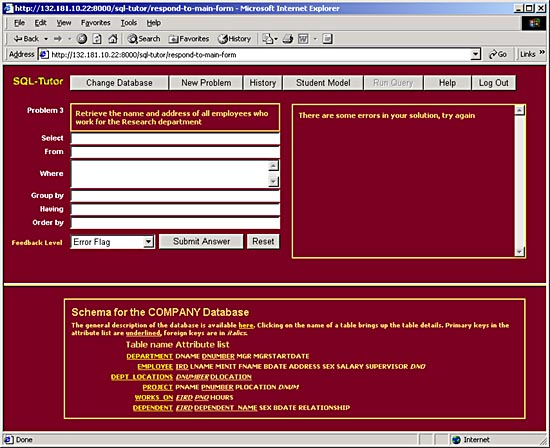
\includegraphics[width=0.8\textwidth]{sqlt-web}
\end{center}
\end{figure}

\subsection{Önnur SQL-kennslutól}
\label{sec:other-sql-teaching-tools}
Khan Academy er bandarísk menntastofnun sem ekki er rekin í gróðaskyni. Stofnunin hefur vakið athygli fyrir kennslu byggða á myndböndum, en hún býður meðal annars upp á stutta yfirferð á SQL með SQLite\footnote{\url{https://www.khanacademy.org/computing/computer-programming/sql}}. Auk myndbandanna býður SQL-námskeið Khan Academy nemendum upp á að keyra SQL-skipanir í vafraglugga sínum, á sama sniði og er notað í fyrirlestramyndböndunum. Nemandanum er umbunað með stigum fyrir framgang sinn í myndbandaáhorfi og æfingum. Nemandinn er leiddur með fastmótuðum hætti í gegnum námsefnið - þó að nemandinn geti stjórnað hraða sínum sjálfur eru ekki mikil tækifæri til sjálfstæðrar könnunar. Uppbygging efnisins er miðuð að sjálfsnámi nemenda, þeir hlutar kerfisins sem snúa að kennurum og samskiptum þeirra við nemendur eru seinni tíma viðbætur.

Kerfi sem hefur verið notað til stuðnings í Tækniskólanum er SQLZoo\footnote{\url{http://sqlzoo.net/}}. Um ``interactive tutorial'' er að ræða, þar sem nemandanum gefst kostur á að vinna sig í gegnum sífellt flóknari verkefni. Hægt er að framkvæma SQL-skipanir á vefsíðunni sjálfri, með tafarlausri endurgjöf. Síðan er byggð á MediaWiki og hún þar með opin fyrir breytingum utanaðkomandi aðila.
Líkt og í mörgum öðrum kennslukerfum samanstendur SQLZoo fyrst og fremst af æfingum í að framkvæma fyrirspurnir. Upplýsingum er ekki gefið samhengi, heldur er nemandanum strax beint að því að fara að skrifa SQL-skipanir. Framvindan í gegnum námsefnið er fyrst og fremst línuleg.

Schemaverse\footnote{\url{https://schemaverse.com/}} er leikur fremur en kennslutól, en leikurinn er spilaður með því að framkvæma SQL-skipanir til að stjórna ``geimskipum'' sem keppa við geimskip annarra. Möguleiki er á að nota leikinn til þjálfunar fyrir lengra komna nemendur og þá sem hvattir eru af samkeppni.

Nemendur sem vilja sækja formlegra netnámskeið hafa úr mörgu að velja. Coursera\footnote{\url{https://www.coursera.org/}} og edX\footnote{\url{https://www.edx.org/}} bjóða bæði upp á fjölmörg námskeið sem tengjast gagnagrunnum.

\subsubsection{Greining}
Óakademísku tólin mynda fjölbreyttari hóp en þau akademísku. Sum eru hluti af breiðu námsúrvali ósérhæfðari menntastofnunar (Khan Academy), önnur bera þess merki að vera búin til af einstaklingum eða fámennum hópi í gróðaskyni (SQLZoo) og önnur jafnvel sem áhugamál (Schemaverse).

Framsetning er í sumum tilfellum gríðarlega markviss, eins og við má búast af kerfum sem ekki geta gengið að nemendahóp vísum. Stærri síðurnar (Coursera, edX, Khan Academy) eru nútímalegar og vel hannaðar, SQLZoo er með áberandi stutta leið frá forsíðu að SQL-æfingum. Munurinn er sérlega sláandi þegar þau eru borin saman við akademísku tólin sem eru ekki einu sinni aðgengileg á netinu og bera þess vott að njóta ekki reglulegra viðmótsuppfærslna, sjá \myref{fig:sqltutorweb}.

Endurgjöf er jákvæð - Khan Academy gefur stig, SQLZoo gefur glaðlega broskalla þegar æfingu er lokið. Verið er að búa til hvata fyrir nemendur til að halda áfram þegar ytri þrýstingur (á borð við hættuna á að falla í námskeiði) er ekki endilega til staðar.

Opnu tólin þjást að mati höfundar helst af annars vegar stefnuleysi og hins vegar skorti á möguleikum til að þætta tólið saman við hefðbundna kennslu. Tólin þurfa að geta þjónað mjög breiðum hópi nemenda til að viðhalda vinsældum sínum, sem takmarkar þau í að bjóða upp á sérhæft efni. Tólin eru miðuð að nemendum sem stunda sjálfsnám, kennarar sem hyggjast nýta þau í kennslustofu þurfa að nota óbeinar aðferðir til að fylgjast með og taka þátt í framgangi nemenda.

Af velgengni þeirra má læra, en kennsluvefur sem hefur það sérstaka hlutverk að styðja við kennslu í hefðbundnu námskeiði þarf að hafa aðrar áherslur.
\chapter{Hugmyndafræði}
Mýmargar leiðir eru til að læra SQL á netinu í dag. Eigi að vera gagn af því að búa til einn vefinn enn þarf því að velja áhersluatriði til að mynda sérstöðu. Þau sem valin voru við smíði þessa kennsluvefs eru: 
\begin{itemize}
 \item Notkun á vefnum til framsetningar á bókartexta \myref{sec:web-as-book}
 \item Samtvinnun texta og æfinga \myref{sec:exercise-explanation}
 \item Opin hugmyndafræði sem vörn gegn úreldingu \myref{sec:durability}
\end{itemize}

\section{Vefurinn sem bók}
\label{sec:web-as-book}
Forveri verkefnisins er kennslubók. Bókin var gefin út rafrænt, en nýtti sér þó þá kosti sem slíkt fyrirkomulag hefur í för með sér ekki nema að takmörkuðu leyti. Innri og ytri tenglar voru til staðar í bókinni, en að flestu öðru leyti var um nokkuð hefðbundið rafrænt skjal að ræða.

Kennsluvefurinn er hugsaður sem ítrun, eða næsta útgáfa, á rafrænu kennslubókinni. Ekki er um að ræða endurskrift frá grunni, heldur er ætlunin að endurnýta það sem gefist hefur vel og bæta við virkni sem ekki var mögulegt að útfæra sem hluta af .pdf skjalinu. 

Nálgunin er því með öðrum hætti en á öðrum SQL-kennslusíðum, til dæmis SQLZoo eða Khan Academy \myref{sec:other-sql-teaching-tools}, þar sem nemandanum er annars vegar beint í átt að æfingaverkefnum og hins vegar í átt að kennslumyndböndum. Áhersla kennsluvefsins er sem sagt eftir sem áður á framsetningu á ``gamaldags'' efnistexta.

Venjulegur texti hefur ýmsa kosti í för með sér. Þeir sem voru höfundi efst í huga eru þó helst eftirfarandi:

\begin{itemize}
 \item Aukinn möguleiki á að nýta eldra efni
 \item Auðveldari uppfærslur, sjá endingargildi \myref{sec:durability}
 \item Auðveldari samþætting efnis frá öðrum höfundum, sjá opið efni \myref{sec:open-material}
\end{itemize}

Þekktasta dæmið um síðu sem hefur verið unnin með þessum hætti er Wikipedia\footnote{\url{https://www.wikipedia.org/}}, sem ekki þarfnast kynningar. Sú síða hóf göngu sína sem ítrun á hugmyndinni um alfræðiorðabók og ber hún þess merki. Aðalefni síðunnar er enn á textasniði. Myndbönd og hljóðefni eru í aukahlutverki og framsetning efnisins er með aðskildum greinum sem vísa hver í aðra. 

Þó að áhersla sé á að varðveita nokkur af betri einkennum kennslubóka eru tvö atriði sem sérstaklega var lagt upp með að bæta við. Þau eru gagnvirkar æfingar \myref{sec:exercise-explanation} og markviss ólínuleg framvinda \myref{sec:nonlinearity}.

\subsection{Ólínuleg framvinda}
\label{sec:nonlinearity}
Hefðbundin kennslubók, hvort sem hún er sett fram á pappírsformi eða rafrænu, birtir lesandanum efnistexta sinn í fastri röð. Þetta er eðlileg skorða sem fylgir pappírsbókum - þegar geyma á texta á pappír er hann geymdur á aðskildum blaðsíðum. Sumar bækur innihalda fram- og bakvísanir með blaðsíðunúmerum, en vegna þess hve erfitt er að finna nákvæma blaðsíðu eftir blaðsíðutali eru flestar bækur þannig upp byggðar að blaðsíðunum er gert að lesa þær í vaxandi röð eftir blaðsíðutali. Við gerð námsbóka hefur þessi ``línulega'' tilhögun mikilvægan kost, nefnilega þann að á hverri blaðsíðu er hægt að gera ráð fyrir að lesandinn hafi lesið allar blaðsíður sem á undan koma. 

Þessi skilyrði hljóma auðvitað sjálfsögð, en koma greinilega fram þegar efnisframsetning í kennslubókum er bornar saman við þá sem finna má í sjálfstæðum greinum. Og sjálfstæðar greinar eru það snið sem upplýsingar á vefnum eru aðgengilegar á nema sérstakar og kauðalegar rástafanir séu gerðar til að koma í veg fyrir það.

\begin{figure}
\caption[Samanburður á línulegri og ólínulegri framvindu]{Samanburður á línulegri og ólínulegri framvindu. Til vinstri: Efnisatriði um netafræði í kennslubók (Discrete Mathematics and its Applications, Rosen 2011), sett fram í röð. Til hægri: Efnisatriði um netafræði sett fram í merkingarlausri röð á upplýsingasíðu um stærðfræði (ProofWiki\footnotemark).}
\begin{center}
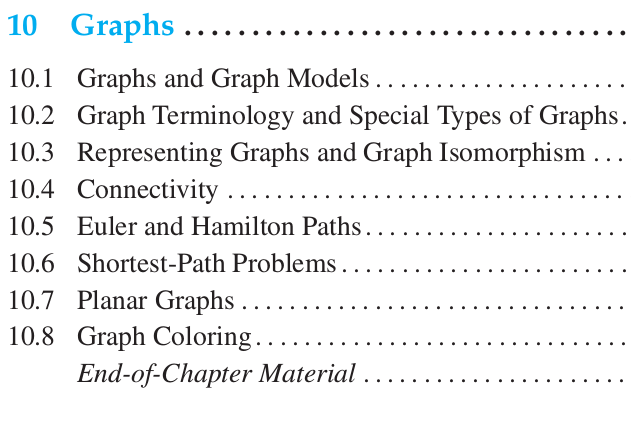
\includegraphics[height=5cm]{ordered-progression}
\hspace{1cm}
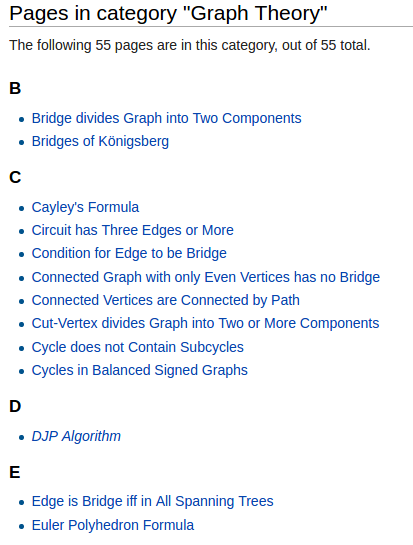
\includegraphics[height=5cm]{unordered-progression}
\end{center}
\end{figure}
\footnotetext{\url{https://proofwiki.org/wiki/Category:Graph_Theory}}

Almennt er hægt að komast að grein á veraldarvefnum með því að fylgja einkvæmri vefslóð. Tengill á þá vefslóð gæti verið hvar sem sem á veraldarvefnum, efnishöfundur getur ekki gert ráð fyrir neinu um hvaða texta lesandinn las síðast né heldur hvaða samhengi upplýsingarnar sem í greininni eru eru settar fram í. Þessi tilhögun auðveldar leit og uppflettingu til muna. Mjög auðvelt er að vísa í grein með slóð og leitarvélar gera auðvelt að leita að grein eftir efnisorðum. Þessir eiginleikar eru góðir fyrir uppflettirit, en eðlislægi skorturinn á línulegri framvindu getur valdið vandræðum.

Það að efnishöfundur vefgreinar viti lítið um samhengið sem greinin er lesin í setur viðkomandi í erfiða stöðu. Höfundur getur gert ráð fyrir að lesandinn viti ``lítið'' um viðfangsefnið og hafið grein sína á að taka fyrir grunnatriði sem nauðsynlegt er að þekkja áður en að efninu sjálfu er komið, eða gera ráð fyrir að lesandinn viti ``mikið'' og undið sér beint að efninu. Í fyrra tilfellinu er hætt við að fróðir lesendur þreytist, í því seinna að verr undirbúnir lesendur tapi þræðinum. Efnishöfundur vefgreinar þarf að taka þessa ákvörðun í hvert skipti sem ný grein er skrifuð, en bókarhöfundurinn þarf einungis að ákveða svið bókarinnar einu sinni.

Þetta vandamál ágerist síðan enn frekar þegar nota á vef til kennslu. Ef setja á lesefni í námskeiði fram sem safn sjálfstæðra vefgreina, þá stendur valið á milli þess að skipuleggja greinar um seinni viðfangsefni námskeiðsins þannig að þær útskýri í sífellu grunnatriði úr fyrri greinum sem nemandinn gæti eða gæti ekki hafa lesið - eða þá skilgreina fyrir greinarnar einhvers konar röðun.

Skilgreining röðunar fyrir vef er ekki sérstaklega einföld. Það að einfaldlega númera greinarnar og tilskipa að þær skuli lesa í ákveðinni röð brýtur gegn eiginleikum veraldarvefsins, að hvaða grein sem er sé í eðli sínu aðgengileg hvaðan sem er. 

Sú leið sem farin er á þessum kennsluvef til að tengja greinarnar saman er að skilgreina ráðgefandi vensl á greinarnar.
\subsubsection{Venslaðar greinar}
Á kennsluvefnum er námsefninu raðað niður á greinar. Greinar geta verið mislangar, en hver þeirra ætti að innihalda útskýringu á efnisatriði sem myndar eina heild - safn af texta sem á heima undir sameiginlegri fyrirsögn. Hugmyndinni um ``kafla'' er haldið nokkuð óbreyttri frá þeirri sem við þekkjum úr pappírsbókum, greinum sem fjalla um sama efni er ennþá safnað saman þó röðin á milli þeirra sé skilgreind með öðrum hætti.

Til að leiða nemendur á milli greina eru skilgreindar á milli þeirra tengingar. Hver grein hefur þannig skilgreindar ráðleggingar um hvað skuli lesa næst eftir að lestri greinarinnar er lokið. Þetta gæti verið ein grein sem er fyrirkomulagið sem hefðbundið er í pappírsbók, margar greinar eða engin.
\begin{figure}
\caption{Tengsl greina á kennsluvefnum}
\label{fig:force-direction}
\begin{center}
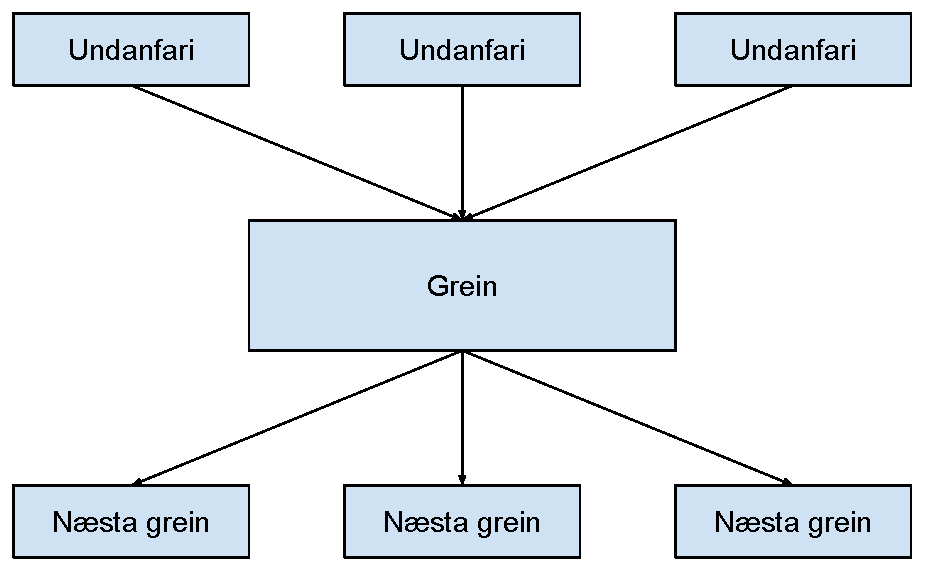
\includegraphics[width=0.6\linewidth]{Undanfarar}
\end{center}
\end{figure}
Hugmyndin er að þessar skilgreindu tengingar myndi milliveg milli línulegrar handleiðslu, sem hefðbundnar bækur bjóða upp á, og þess algjöra frelsis sem nemandi sem nýtir sér leitarvélar hefur. Nemandanum er gefið nokkuð val um í hvaða röð viðkomandi vill kynna sér efnið og er hvattur til könnunar, án þess að eiga það á hættu að villast af leið yfir í framandi efni.

Efnishöfundurinn hefur áfram mikið vald til að ákvarða ráðlagða lesröð á greinum. Í útfærslunni ákveður efnishöfundur eina grein í hverjum kafla sem lesandanum er ráðlagt að lesa fyrst, ásamt því að ákveða tengingarnar á milli greinanna. Þar sem tengingarnar eru aðalleiðin til að ráfa um kennsluefnið getur höfundurinn haft nokkra hugmynd um hvaða greinar hafa verið lesnar áður en að hverri grein er komið - sem auðveldar umfjöllun til muna.

Fyrirkomulagið er ekki gallalaust. Hönnun samkvæmt er erfitt að fletta upp í vef sem settur er upp á þennan hátt, leitarvélar eru ekki studdar sérstaklega og notkun þeirra felur í sér ákveðna sniðgöngu á ráðleggingarkerfinu. Auk þess er hætta á að lesandinn ``týnist'' í ferðalagi sínu um efnið sé ekki um venjulegt blaðsíðutal að ræða. Til að koma í veg fyrir þetta eru vensl greinanna sett fram myndrænt með notkun neta. Nánar um útfærslu má sjá í \ref{sec:d3js}.
\begin{figure}
\caption{Dæmi um tengsl greina, sett fram með stefndu neti.}
\begin{center}
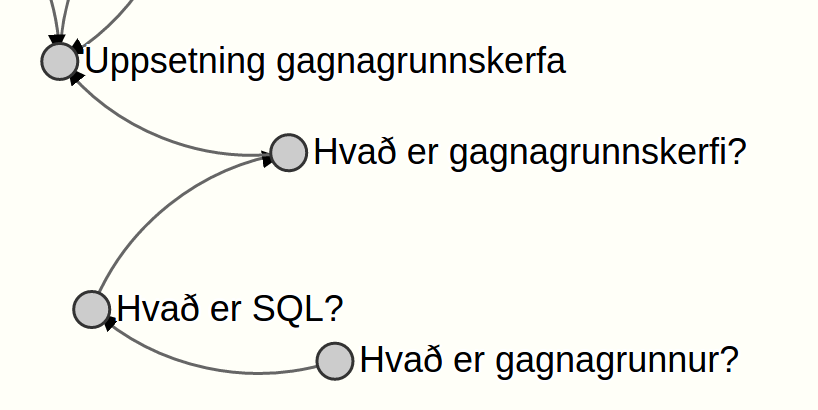
\includegraphics[width=0.8\textwidth]{relational-sections}
\end{center}
\end{figure}

Auk þess sem hverja grein má tengja við aðrar greinar má líka vísa í æfingar út frá greinum.
\section{Æfingar}
\label{sec:exercise-explanation}
Viðfangsefni þessa tiltekna kennsluvefs er kennsla í notkun SQL, sem er í eðli sínu verkleg. Æfingar eru því mikilvægur og sjálfsagður þáttur námsefnisins.

Vefbók hefur þann kost að hægt er að sameina texta og forritunaræfingaumhverfi á mun nánari hátt en í venjulegum rafbókum. Venjuleg rafbók er fyrst og fremst skjal sem hægt er að lesa, vefur er forrit sem getur boðið upp á gagnvirkni.

Kennsluvefurinn hefur innbyggt æfingasvæði þar sem nemandinn getur leyst fyrirfram skilgreindar SQL-æfingar. Nemandinn getur framkvæmt ýmsar gerðir SQL-skipana, sem eru metnar sjálfkrafa.

Áhersla var lögð á að æfingar falli mjúklega inn í efnisumfjöllunina. Hægt er að tengja hverja grein vefsins við æfingu eða æfingar, auk þess sem vísa má til þeirra inni í textanum með venjulegum veftenglum. Viðmót æfingaumhverfisins er gert sem líkast viðmóti vefsins sjálfs til að lágmarka truflandi áhrif þess að ``skipta um umhverfi''. Hugmyndin er sú að upplifun nemandans sé ekki að fyrst þurfi að lesa upplýsingatexta og svo leysa æfingar, heldur myndi textinn og æfingarnar samstæða heild.

Sjá má meira um æfingaumhverfið og útfærslu þess undir \myref{sec:command-analysis}.

\section{Endingargildi}
\label{sec:durability}
Kerfi byrja að úreldast um leið og þau eru gefin út. Án stöðugs viðhalds höfunda brotna þau niður og hverfa, breytast í sögudæmi. Slík viðhaldsvinna er erfið og dæmin\cite{bhagat2002, mitrovic2003intelligent, sadiq2004sqlator} sanna að ekki er hægt að reiða sig á að hún haldi áfram eftir áratug.

Til að sporna við hnignun þessa kennsluvefs eftir að höfundur mun eðlilega og óumflýjanlega hverfa til annarra starfa er leitað í hugmyndasmiðju opins hugbúnaðar (e.\ \emph{open source software}). Kennsluvefurinn er opinn á þrenna vegu - kennsluefni vefsins er opið, grunnkóði vefsins er opinn og allur hugbúnaður sem vefurinn byggir á er líka opinn.
\subsection{Opinn kóði}
\label{sec:open-source}
Allur grunnkóði vefsins er opinn og aðgengilegur á Github-síðu höfundar\footnote{\url{https://github.com/Ernir/sql-web}}. Hver sem er getur skoðað kóðann og sett hann upp á sinni vél og breytt honum að vild, í samræmi við skilmála opins kóðaleyfis \myref{sec:license} sem dreift er með kóðanum. Kóðanum er dreift með Git\footnote{\url{https://git-scm.com/}} útgáfustjórnunarkerfinu, sem er sérstaklega hannað til að virka án miðlægs vefþjóns. Endingargildi kerfisins er þar með aukið umfram það sem höfundur gæti boðið upp á - kerfið mun lifa svo lengi sem einhver sem sótt hefur kóðann heldur honum aðgengilegum og uppfærslur munu geta borist svo lengi sem kerfið er í notkun.

Það að hver sem er geti sett upp keyrandi útgáfu af kennsluvefnum myndar líka hornsteininn í dreifingarmöguleikum kerfisins. Vefurinn er ekki takmarkaður við eina, skilgreinda útgáfu sem stjórnað er af höfundi, heldur getur hver skóli eða jafnvel hver áfangi, keyrt sína eigin sérsniðnu útgáfu. Til dæmis gefur þetta möguleika á að sérsníða afkastagetu vefsins, skóli með smáar þarfir getur notast við einfalda, ódýra vefhýsingu en stærri skóli gæti tileinkað vefnum heilan vefþjón.

Höfundur hyggst halda úti grunnútgáfu af vefnum sem verður aðgengilegur á léni í eigin eigu. En fari svo að höfundur hverfi frá verkefninu og sú útgáfa sem á því léni verði aftend er vefurinn sjálfur þar með ekki dauður og gleymdur - allar aðrar útgáfur munu áfram virka og grunnkóðinn verður enn til.

Allar tæknilausnir frá þriðja aðila sem vefurinn notar eru einnig opnar og ókeypis. Sömu rök um endingargildi eiga því líka við um þær, ekki er hætta á að undirstöður vefsins hverfi undan honum. Um þær tæknilausnir má lesa nánar í \myref{sec:third-party-tech}.
\subsection{Opið efni}
\label{sec:open-material}
Kóðanum og efninu sem vefurinn inniheldur er dreift samhliða og með svipuðum aðferðum. 
Meðal afleiðinga þess er að allt efni vefsins er breytanlegt af notendum hans, í samræmi við skilmála opins efnisleyfis \myref{sec:license}. Sérstakar viðbætur \myref{sec:markdown-additions} voru gerðar til að gera efnissmíði við hæfi kennsluvefsins auðveldari.

Hver kennari getur þannig bætt við ``köflum'' í bókina, falið hluta efnisins og framkvæmt hverjar þær áherslu- og efnisbreytingar sem viðkomandi þóknast.
Þetta mætti til dæmis nota til að bæta við stuðningi við nýtt gagnagrunnskerfi eða til þess að fella sérsniðin myndbönd inn í textann.

Fyrirkomulagið hefur sömu afleiðingar fyrir endingargildi efnisins og opna kóðafyrirkomulagið hefur fyrir endingargildi vefsins sjálfs. Efnið mun halda áfram að þróast svo lengi sem áhuginn á því lifir.
\chapter{Útfærsla vefsins}
Vefsíður eru ekki skrifaðar vélamálsskipun fyrir vélamálsskipun frekar en önnur forrit á 21. öldinni, þær nota verk annarra forritara. Byggja ofan á sum forrit, öðrum forritum má breyta og bæta svo hægt sé að innlima þau í ný forrit. 

Þeim forritum frá þriðja aðila sem koma við sögu \myref{sec:third-party-tech} og þeim forritshlutum sem vinna nýju, markverðu vinnuna \myref{sec:homemade-tech} þarf að gera skil.
\section{Aðfengnar tæknilausnir í notkun}
\label{sec:third-party-tech}
Vefurinn er skrifaður með Django \myref{sec:django}, sem er sú tæknilausn frá þriðja aðila sem mest einkennandi er fyrir útfærslu vefsins. Efni vefsins er skrifað með Markdown \myref{sec:markdown}. Auk þess eru framendapakkarnir Tufte CSS \myref{sec:tufte-css} og D3.js \myref{sec:d3js} notaðir til að stýra útliti vefsins.
\subsection{Django}
\label{sec:django}
Django er vefburðargrind (e.\ \emph{web framework}) fyrir Python-forritunarmálið. Slík burðargrind veitir meiri stuðning en bein Python-forritun gegn vefþjóni, en mun minni stuðning en vefumsjónarkerfi eins og WordPress. Django var fyrst gefið út árið 2005 af Adrian Holovaty og Simon Willison, sem þróuðu kerfið út frá forritum sem þeir höfðu notað við netblaðaútgáfu. Það er mest notaða Python vefburðargrindin í dag.

Django fylgir Model-View-Controller (MVC) hönnunarmynstrinu eins og það er venjulega túlkað á vefnum. Flest ``fyrirbrigði'' kennsluvefsins eru þannig skilgreind af Python-forritsklösum sem tengjast hlutvenslakerfi (e.\ \emph{object-relational mapping, ORM}) grindarinnar \myref{sec:django-orm}.

Burðargrindin hjálpar einnig stórlega við kóðaendurnýtingu og framsetningu. Sem dæmi má taka að stílsupplýsingar sem eru öllum undirsíðum kennsluvefsins sameiginlegar má finna í einni grunnskrá \myref{code:base-template}.
\subsubsection{Hlutvenslakerfi}
\label{sec:django-orm}
Hlutvenslakerfi kerfi Django heldur utan um gagnagrunnstengingar og upplýsingar sem viðkoma Django-vefsíðu.

Kerfið er hlutbundið. Klasi sem táknar ``fyrirbrigði'' í Django erfir frá \texttt{model} klasa gefnum af burðargrindinni. Forritarinn bætir síðan við eigin eiginleikum og aðferðum sem viðkoma forritinu. Burðargrindin sér um að smíða gagnagrunnstöflur sem geymt geta þær upplýsingar sem þarf til að tákna tilvik af klasanum.

Vensl á milli fyrirbrigða skilgreinast líka af hlutvenslakerfinu. Þannig er hugtakið \texttt{Section} til dæmis tengt við hugtakið \texttt{Excercise} með eiginleikanum \texttt{associated_exercises} sem skilgreindur er í \texttt{Section} klasanum og vísar á \texttt{Exercise} klasann með nafni, sjá kóðalistun \myref{code:orm-example}. Allir \texttt{model} klasar sem viðkoma kennsluvefnum eru skilgreindir í skránni \texttt{sql\_web/models.py} \myref{code:django-model-objects}.

\begin{listing}
\caption[Tengsl skilgreind með Django hlutvenslakerfinu]{Hluti Section klasans, vensl milli ``Section'' og ``Exercise'' skilgreind}
\label{code:orm-example}
\begin{minted}[frame=lines]{python}
class Section(models.Model):
    """..."""
    associated_exercises = models.ManyToManyField("Exercise")
    """..."""
\end{minted}

\end{listing}


\subsection{Markdown}
\label{sec:markdown}
Greinar kennsluvefsins eru skrifaðar í ívafsmálinu (e.\ \emph{markup language}) Markdown\footnote{\url{http://daringfireball.net/projects/markdown/}}. Markdown er mikið notað, líklegt er að kennarar í tölvugreinum hafi rekist á afbrigði af Markdown á síðunum Github\footnote{\url{https://github.com/}}, Stack Overflow\footnote{\url{http://stackoverflow.com/}} eða á spjallborði á netinu.

Aðaláhersluatriði Markdown er að frumkóði (e.\ \emph{source code}) textaskjalsins sé læsilegur og auðskrifanlegur. Þetta er ólíkt þekktasta ívafsmálinu, HTML, þar sem markmiðið er að skilgreina einingar til framsetningar. HTML inniheldur þess vegna töluverðar viðbótarupplýsingar um hvernig birta skal textann, sbr. mynd \myref{fig:markdown} sem eru áskildar í Markdown.

\begin{figure}
\caption{Upprunalegur Markdown-kóði og HTML-ið sem hann skilgreinir}
\label{fig:markdown}
\begin{center}
\texttt{Markdown styður *skáletrun*}

$\downarrow$

\texttt{<p>Markdown styður <em>skáletrun</em></p>}

\end{center}
\end{figure}

Markdown-sniðið er sem sagt sérstaklega hannað til að skrifa texta án truflana, sem svo er oft þýddur yfir í þyngri ívafsmál með þar til gerðu forriti. Markdown-málið er upphaflega skilgreint óformlega með slíku forriti, Perl-forritinu \texttt{Markdown.pl} sem þýðir markdown yfir í HTML, skrifað af John Gruber árið 2004. Kennsluvefurinn notar Markdown á hliðstæðan hátt, tekið er við Markdown-texta frá efnishöfundi og hann þýddur yfir á HTML með Markdown-túlki. Markdown-útfærslan sem kennsluvefurinn notar er Markdown-pakki Python forritunarmálsins\footnote{\url{https://pypi.python.org/pypi/Markdown}}.

Sérstakar viðbætur voru gerðar við Markdown-pakkann til að styðja sérkröfur kennsluvefsins \myref{sec:markdown-additions}.
\subsection{D3.js}
\label{sec:d3js}
Til að sýna vensl á milli greina er gagnaframsetningarforritunarsafnið D3.js\footnote{\url{https://d3js.org/}} notað. Um er að ræða Javascript-safn.

Safnið er stórt og almennt, hægt er að nota það við vinnslu og til birtingar á alls kyns gögnum. Hér er það notað til að sækja upplýsingar um vensl greina frá bakenda (með AJAX) og til að birta yfirlitsmyndir fyrir upplýsingarnar.

Yfirlitsmyndirnar eru búnar til með því að skilgreina hverja grein sem hnút í neti, vensl þeirra á milli með örvalegg, og framkvæma síðan tvívíða eindahermun. Hver hnútur er meðhöndlaður sem neikvætt hlaðin eind, hverjum legg úthlutað lengd og teygjanleika og eindasafnið látið dreifa úr sér í tvívíðri sléttu. Þessi hegðun fæst fyrirhafnarlítið frá D3.js, en hjartað í hermuninni má sjá á kóðalistun \myref{code:force-direction}. Niðurstöðurnar eru á mynd \myref{fig:force-direction}.

\begin{listing}
\caption[Eindahermun með D3.js]{Hluti eindahermunarinnar sem framkvæmd er með D3.js. Hnútar með neikvæða hleðslu og leggir með lengd eru skilgreindir. Hermunin er uppfærð við hvern ``tick'' viðburð og hún sett í gang.}
\label{code:force-direction}
\begin{minted}[frame=lines]{js}
var force = d3.layout.force()
    .nodes(d3.values(nodes))
    .links(links)
    .size([width, height])
    .linkDistance(80)
    .charge(-300)
    .on("tick", tick)
    .start();
\end{minted}

\end{listing}


\subsection{Tufte CSS}
\label{sec:tufte-css}
Þar sem kennsluvefurinn skal virka sem vefútgáfa af bók er mikilvægt að huga að framsetningu textans.

Það sem helst einkennir útlit vefsins er notkun á css-safninu Tufte CSS\footnote{\url{https://github.com/edwardtufte/tufte-css}}. Safnið er hannað út frá hugmyndum fræðimannsins Edward Tufte um framsetningu texta.

Meðal einkennandi atriða fyrir stíl Tufte er áberandi notkun spássíugreina og mikil samþjöppun texta og mynda, sjá mynd \ref{fig:tufte-example}. Þær viðbætur sem gerðar eru við Markdown-pakkann \myref{sec:markdown-additions} eru einkum til að styðja við þessi sérstöku textaatriði.

\begin{figure}
\caption{Spássíugreinar og myndir í stíl Tufte.}
\label{fig:tufte-example}
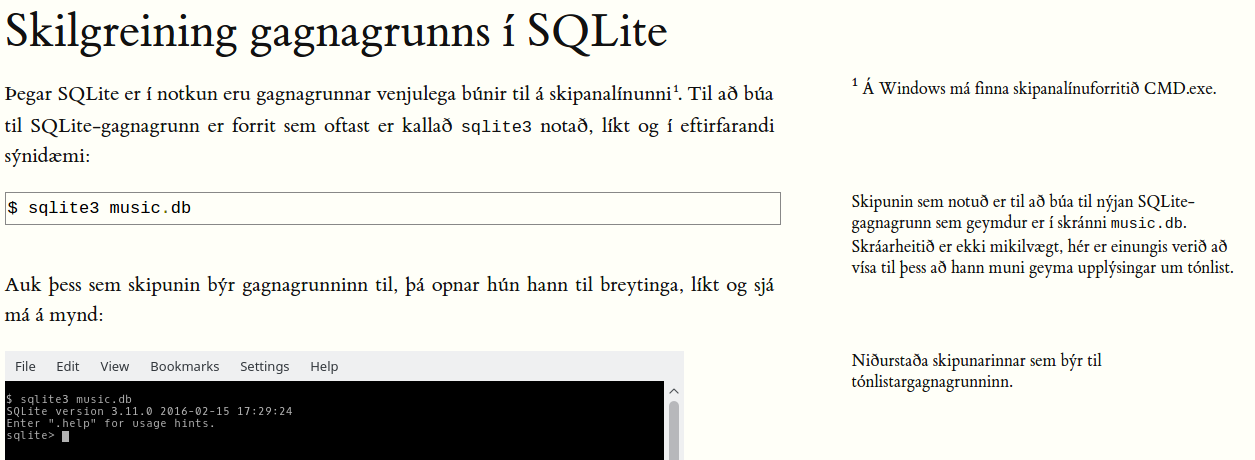
\includegraphics[width=\textwidth]{tufte-example}
\end{figure}

\section{Sérsmíðaðar tæknilausnir}
\label{sec:homemade-tech}
Töluverð forritun liggur að baki sérhæfðum vef. Mikið af forrituninni er handavinna sem liggur að baki flestum nútímavefsíðum, en á þessum vef eru líka atriði sem skoða má sérstaklega. Hér eru það annars vegar forritseiningar sem greina SQL-fyrirspurnir \myref{sec:command-analysis} og hins vegar Markdown-viðbætur \myref{sec:markdown-additions}.
\subsection{Greining á SQL-skipunum nemenda}
\label{sec:command-analysis}
Ólíkt fyrri kennslutólum sem leggja mikla áherslu á að greina nemendafyrirspurnir\cite{mitrovic1998, bhagat2002} leggur kennsluvefurinn áherslu á framsetningu efnisins. Í samræmi við þá áherslu eru þau tól sem vefurinn notar til að greina fyrirspurnirnar einföld í samanburði.

Til að keyra SQL-skipun þarf nemandinn að leysa svokallaða æfingu. Æfing (e.\ \emph{exercise}) í kennsluvefnum er skilgreind af Django \myref{sec:django} \texttt{model} hlut, sjá \texttt{Exercise} klasann \myref{code:django-model-objects}. Slíkur hlutur hefur nokkra eiginleika sem vert er að nefna:

\begin{itemize}
 \item Nafn, auðkenni og lýsingu
 \item Gerðarlýsingu (e.\ \emph{schema}) ásamt gögnum, sem sett er upp áður en skipanir eru keyrðar
 \item SQL-skipun sem ætlunin er að láta nemandann líkja eftir
 \item Sjálfgefna skipun, sem nemandinn skal breyta
 \item Tilgreiningu á ``gerð'' æfingarinnar - \texttt{SELECT} æfing eða annars konar æfing
\end{itemize}

Þessir eiginleikar, að viðbættri SQL-skipun sem nemandinn skrifar inn, mynda eina keyrslu á æfingu. Keyrsla á æfingu skilar sanngildi sem tilgreinir hvort SQL-skipun nemandans hafi verið rétt miðað við gefnar forsendur, ásamt skilaboðum til nemandans.

Keyrsla er framkvæmd í skránni \texttt{sql\_web/sql\_runner.py} \myref{code:example-runner}. Hún fer fram í nokkrum skrefum. Ávallt eru grundvallarathuganir gerðar á inntaki notandans, athugað er hvort að breytingar hafi verið gerðar á sjálfgefnu skipuninni og hvort einhver skipun hafi verið slegin inn yfir höfuð. Önnur skref eru mismunandi eftir því hvort að um \texttt{SELECT}-skipun sé að ræða eða ekki.

\subsubsection{Mat á SELECT skipunum}
\label{sec:select-analysis}
Þegar um \texttt{SELECT}-skipanir er að ræða er möguleiki á að sannreyna niðurstöðurnar á sveigjanlegri máta.

Í slíkum æfingum er gerðarlýsingin sett upp og fyrirspurnirnar, bæði fyrirspurn nemandans og samanburðarfyrirspurnin, keyrðar á henni. Út úr þeim keyrslum koma tvö mengi niðurstaðna sem hægt er að bera saman, annars vegar ``nemendamengi'' og hins vegar ``samanburðarmengi''. Séu mengin eins er nemendaskipunin talin rétt.

Gagnagrunnsviðmótið skilar niðurstöðumengjunum sem listum (e.\ \emph{lists}) af línum (e.\ \emph{tuples}). Þessar gagnagrindur (e.\ \emph{data structures}) eru almenns eðlis, sem setja möguleikum á samanburðum nokkrar skorður.

Samanburðurinn fer fram með eftirfarandi hætti:
\begin{itemize}
 \item Athugað er hvort að mengin séu af sömu stærð, séu þau það ekki er samanburðinum strax hafnað
 \item Ítrað er yfir samanburðarmengið og leitað að tilsvarandi stökum í nemendamenginu
 \begin{itemize}
  \item Stökin eru fjarlægð úr tilsvarandi mengjum við samanburðinn
  \item Keyrslu er hætt finnist stak ekki í nemendamenginu
  \item Sé samanburðarmengið myndað með fyrirspurn sem inniheldur \texttt{ORDER BY} er sú krafa gerð að stakið sé fremst í nemendamenginu
 \end{itemize}
 \item Samanburðurinn á milli mengjanna er sannur ef ítrunin tæmir þau bæði.
\end{itemize}

\begin{table}
\caption[Tímaflækja samanburða]{Tímaflækja samanburða á fyrirspurnamengjum í æfingum kennsluvefsins}
\label{tab:comparison-complexity}
\begin{center}
\begin{tabular}{lc}
\toprule
Aðgerð&Tímaflækja í versta tilfelli\\
\midrule
Staðfesting á misstórum mengjum& $O(1)$\\
Samanburður á óröðuðum mengjum& $O(n^2)$\\
Samanburður á röðuðum mengjum& $O(n)$\\
\bottomrule
\end{tabular}
\end{center}
\end{table}
Ítrunin yfir samanburðarmengið tekur línulegan tíma með tilliti til fjölda staka í menginu. Einföld samanburðarleit á borð við þá sem notuð er á nemendamengið er sömuleiðis með línulegan keyrslutíma. Gert er ráð fyrir því að samanburður tveggja lína taki fastan tíma.

Áætlaðar tímaflækjur fyrir samanburði niðurstaðanna má sjá á töflu \myref{tab:comparison-complexity}. Nokkur tímasparnaður næst fram á röðuðum mengjum, þar sem ekki þarf að renna í gegnum allt nemendamengið á hverri ítrun yfir samanburðarmengið. 

Tímaflækja samanburðanna er slæm þegar bera þarf saman tvö óröðuð, jafn stór mengi. Þetta olli áhyggjum vegna þess að samanburðarreikniritið er keyrt að beiðni notenda, sem þarf að bíða eftir niðurstöðunni. Niðurstöðurnar þurfa því að berast mjög hratt, útreikningarnir mega ekki bæta verulega við venjulegan hleðslutíma vefsíðunnar. Prófanir á sýnidæmum hafa ekki bent til slíkra vandræða við raunverulegar aðstæður, þar sem stærð gagnasettanna takmarkast af því að nemendur þurfa að geta meðtekið þau.

Aðferðin hefur auk þess nokkra kosti sem gera hana áreiðanlegri en fyrirsjáanlegir möguleikar á að nota skilvirkari aðferðir.

\paragraph{Aðrar leiðir til að framkvæma samanburði} Þekkt er að hægt sé að bera saman tvö mengi á línulegum tíma með tilliti til fjölda staka sé uppfletting möguleg á föstum tíma. Mengi í Python styðja uppflettingu á föstum tíma, að því gefnu að hægt sé að reikna tætivistföng (e.\ \emph{hash values}) fyrir stökin. Þar sem kennari getur útbúið æfingar með flestum gerðum gagna er óáreiðanlegt að gera ráð fyrir miklu um uppbyggingu hverrar línu.

Einnig er hægt að bera saman mengi á $O(n\log n)$ tíma séu stökin raðanleg. Hvoru mengi um sig er þá raðað með samanburðarröðunarreikniriti og stök mengjanna þvínæst pöruð saman í röð. Þessi leið er einnig illfær. Þó að gögn í gagnagrunnum séu jafnan þess eðlis að hægt sé að raða þeim, þá er röðun ekki áreiðanleg nema á þau sé skilgreindur lykil. Ekki er hægt að stjórna sniði nemendafyrirspurnarinnar, svo ákvörðun á lykli fyrir þær fyrirspurnir væri líka óáreiðanleg.

Báðar leiðinar eru skilvirkari en sú sem valin er, en fela í sér möguleikann á ólíklegum en torskildum villum fyrir notendur vefsins.
\subsubsection{SQLite í minni}
Allar SQL-skipanir nemenda sem kennsluvefurinn keyrir eru keyrðar á SQLite gagnagrunni sem einungis er til í minni kerfisins. Þegar meta skal skipun er tómur gagnagrunnur búinn til í minni, gerðarlýsingin sett upp, nemendafyrirspurnin og samanburðarfyrirspurnin keyrð og gagnagrunninum að lokum eytt. Sjá mynd \myref{fig:sql-evaluation-execution}.	

\begin{figure}
\caption{Framkvæmd mats á nemendafyrirspurn}
\label{fig:sql-evaluation-execution}
\begin{center}
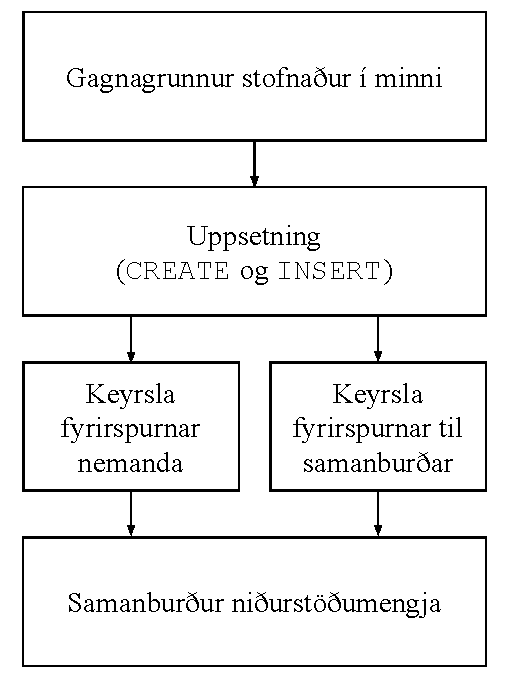
\includegraphics{keyrsla-fyrirspurnar}
\end{center}
\end{figure}

Helsti kostur þessa fyrirkomulags er öryggi. Gagnagrunnurinn er tímabundinn og inniheldur engin gögn nema þau sem eru æfingunni viðkomandi. Tengingin hefur ekki heimildir til að tengjast skráarkerfinu né heldur til að framkvæma SQLite-stýriskipanir (``dot-commands'') sem gætu framkallað breytingar á kerfinu sjálfu eða lesið þaðan upplýsingar. Það er aldrei hættulaust að keyra kóða annars fólks með jafn litlu eftirliti og forritunarkennslukerfi krefst, en með þessum hætti er tekið fyrir algengustu gerðir skaðlegra villna og árása.

Skortur á keyrsluhraða hefur ekki valdið vandræðum með þessu fyrirkomulagi. Þó að það að stofna til nýs gagnagrunns í hvert skipti sem nemandi framkvæmir fyrirspurn feli í sér tímakostnað hefur hann ekki verið greinanlegur. Líklegt er að það að gagnagrunnur í minni krefjist ekki diskaðgangs vegi á móti.
\subsubsection{Mat á skipunum öðrum en SELECT skipunum}
\label{sec:other-command-analysis}
Snúist æfingin ekki um \texttt{SELECT} skipun er strengjasamanburður notaður til að athuga hvort að skipunin sé sambærileg við þá sem herma skal eftir. Samanburðurinn felst í því að Levenshtein-fjarlægð er reiknuð á milli skipananna tveggja. 

Levenshtein-fjarlægð er mælikvarði á hversu líkar tvær runur eru. Í þessu tilviki er um að ræða talningu á því hversu margar eins stafs breytingar þyrfti að gera á streng sem inniheldur fyrirspurn nemandans til að breyta henni í fyrirspurn kennarans.

Fjarlægðin er reiknuð án þess að taka tillit til biltákna (e.\ \emph{whitespace characters}) eða mismunar á milli hástafa og lágstafa. Sé Levenshtein-fjarlægðin á milli strengjanna 0 er skipunin rétt, annars röng. Sé skipunin röng og fjarlægðin lítil er nemandanum birt fjarlægðin, ásamt útskýringu. Markmiðið með að birta Levenshtein-fjarlægðina sé hún lág er til að gefa nemendum vísbendingu um að viðkomandi gæti verið á réttri leið en með smávægilega málskipunarvillu (e.\ \emph{syntax error}), en málskipunarvillur er sá villuflokkur sem nemendur lenda hvað oftast í við að skrifa SQL\cite{ahadi2016students}.

\subsection{Markdown viðbætur}
\label{sec:markdown-additions}
Markdown er einfalt mál og er þar af leiðandi með fáa sérhæfða möguleika tengdum framsetningu textans. Auk þess eru Markdown-túlkar einfeldningsleg textatúlkunarforrit, sem ekki gera sér grein fyrir innri uppbyggingu texta eða tengsla á milli viðfangsefna. Til að styðja myndræna framsetningu og innri tengingar textans er því nauðsynlegt að smíða viðbætur við túlkinn.
 
Opinbera viðbótin \texttt{tables} við Python-pakkann fyrir Markdown er notuð\footnote{\url{https://pythonhosted.org/Markdown/extensions/tables.html}}. Að auki eru fjórar viðbætur skrifaðar sérstaklega fyrir kennsluvefinn. Þær eru: 
\begin{itemize}
 \item Viðbót til að styðja innfellingu mynda (\hyperref[sec:markdown-image-inclusion]{{\color{blue} Myndir}} $\to$ )
 \item Viðbót til að leyfa framsetningu texta í tveimur dálkum með spássíugreinum (\hyperref[sec:markdown-footnote]{\color{blue} Spássíugreinar} $\to$ )
 \item Viðbót til að auðvelda innri tengingu greina (\hyperref[sec:markdown-internal-link]{\color{blue} Innri tenglar} $\to$ )
 \item Smáviðbót til að fegra birtingu kóðadæma innan línu án þess að breyta notkun Markdown
\end{itemize}
Dæmi um útfærslu á viðbót má sjá í \myref{code:footnote-extension}. Hluta af útfærslu má sjá í kóðadæmi \myref{code:markdown-extension-example}.

\begin{listing}
\caption[Skilgreining markdown viðbótar]{Hluti útfærslu á Markdown-viðbót. Hér er reglulegri segð sem þekkir spássíugreinar smeygt á milli innbyggðra segða.}
\label{code:markdown-extension-example}
\begin{minted}[frame=lines]{python}
"""..."""
def extendMarkdown(self, md, md_globals):
    FOOTNOTE_RE = r"\[\^(?P<identifier>[a-z\d#-_]+)\]\[(?P<text>.*?)\]"
    footnote_pattern = Footnotes(FOOTNOTE_RE, self.getConfigs())
    footnote_pattern.md = md
    md.inlinePatterns.add("footnote", footnote_pattern, "<not_strong")
"""..."""
\end{minted}

\end{listing}

\subsubsection{Myndir}
\label{sec:markdown-image-inclusion}
Óbreytt Markdown styður infellingu mynda í texta.
Snið slíkra innfellinga má sjá á málritinu á mynd \myref{fig:markdown-image-inclusion-original}. Hér er \emph{<image-hyperlink>} vefslóð á myndina sem fella skal inn í textann, \emph{<alt-text>} sá texti sem er sýndur í stað myndar sé myndin ekki til staðar og \emph{<title>} viðbótarupplýsingar með myndinni.

\begin{figure}
\caption{Myndainnfellingar í Markdown}
\label{fig:markdown-image-inclusion}
\begin{subfigure}[b]{\textwidth}
\caption{Upprunaleg útgáfa}
\label{fig:markdown-image-inclusion-original}
\begin{syntaxenv}{markdown-image}
  `!' `[' <alt-text> `]' `(' <image-hyperlink> 
  \begin{stack}
  `"' <title> `"'\\
  
  \end{stack}
  `)'
\end{syntaxenv}
\end{subfigure}

\begin{subfigure}[b]{\textwidth}
\caption{Viðbætt útgáfa}
\label{fig:markdown-image-inclusion-enhanced}
\begin{syntaxenv}{enhanced-markdown-image}
  \begin{stack}
  \\
  `f'\\
  `m'
  \end{stack}
  `!' `[' <alt-text> `]' `(' <image-identifier>
  \begin{stack}
  `"' <title> `"'\\
  
  \end{stack}
  `)'
\end{syntaxenv}
\end{subfigure}
\end{figure}

Sérsmíðaða viðbótin, sem vinnur samkvæmt mállýsingu á mynd \myref{fig:markdown-image-inclusion-enhanced}, býður upp á aukamöguleika sem sérstaklega tengjast kennsluvefnum og hans framsetningarmöguleikum.

Athugum að texti kennsluvefsins er settur fram í tveimur dálkum, aðaldálki og spássíudálki, sjá undirkafla \myref{sec:tufte-css}. Fyrst er gefinn möguleiki á að skeyta stafnum \texttt{m} eða stafnum \texttt{f} framan við myndskilgreininguna. Sé stafnum sleppt fyllir myndin aðaldálkinn. Sé stafurinn \texttt{m} gefinn fyllir myndin spássíudálkinn. Sé stafurinn \texttt{f} gefinn fyllir myndin báða dálkana.

Einnig bætast við fleiri möguleikar á að vísa í myndir. Fyrst er reynt að lesa \texttt{<image-identifier>} sem einkvæmt auðkenni Django-model hlutar sem skilgreinir mynd. Finnist engin mynd með viðkomandi auðkenni er leitað að kóðasýnidæmi með auðkennið \texttt{<image-identifier>}. Finnist ekkert kóðasýnidæmi heldur er \texttt{<image-identifier>} notað beint sem vefslóð og er virknin þá sem fyrr.
\begin{listing}
\caption{Möguleg dæmi um myndainnfellingar í Markdown}
\label{fig:markdown-image-examples}
Óbreytt Markdown:
\begin{center}
\texttt{![Alt text](/path/to/img.jpg "{}Optional title")}
\end{center}

Með viðbót:
\begin{center}
\texttt{
 ![Alt text](identifier "{}Optional title")\\
f![Alt text](identifier "{}Optional title")\\
m![Alt text](identifier "{}Optional title")\\
}
\end{center}
\end{listing}

\subsubsection{Spássíugreinar}
\label{sec:markdown-footnote}
Vefurinn gerir ráð fyrir notkun hliðarútskýringa í spássíum.
Sú viðbót sem helst ætti við til að styðja slíka framsetningu væri Footnotes-viðbótin fyrir Python-útgáfuna af Markdown\footnote{\url{https://pythonhosted.org/Markdown/extensions/footnotes.html}}, en hún gerir einungis ráð fyrir hefðbundnum neðanmálsgreinum. Viðbótin var því endurskrifuð.

Viðbótin vinnur samkvæmt mállýsingu á mynd \myref{fig:markdown-footnote}. \texttt{<note-identifier>} er auðkenni sem ekki birtist notanda síðunnar, en má nota til að vísa í spássíugreinina, til dæmis með tenglum. Löglegir stafir í þessu auðkenni skilgreinast af reglulegu segðinni \verb|[a-z\d#-_]|. \texttt{<contents>} myndar eiginlegan texta spássíugreinarinnar, sem má sjálft innihalda Markdown. Hvaða Markdown-texti sem er er sem sagt löglegur, en sterklega er mælt gegn því að setja skilgreiningu á spássíugrein inn í spássíugrein.

\begin{figure}
\caption{Spássíugreinar í Markdown}
\label{fig:markdown-footnote}
\begin{syntaxenv}{markdown-footnote}
  `[' `^' <note-identifier> `]' `[' <contents> `]'
\end{syntaxenv}
\end{figure}

\subsubsection{Innri tenglar}
\label{sec:markdown-internal-link}
Gert er ráð fyrir að tengingar á milli greina séu mikið notaðar innan texta kennsluvefsins. 
Óbreytt Markdown inniheldur almennar leiðir til að fella tengla inn í setningar, en slíkt hefur ókosti í för með sér:

\begin{enumerate}
 \item Breytist vefslóð kennsluvefsins\footnote{Þetta er mjög líklegt að gerist oft, sjá \myref{sec:open-source}} þarf að gera breytingar á frumtextanum til að viðhalda tenglunum
 \item Vefslóðir innihalda mikið af upplýsingum sem eru textahöfundum óviðkomandi
\end{enumerate}
Viðbótin gerir mögulegt að vísa í aðrar greinar kennsluvefsins með því að nota einkvæmt auðkenni viðkomandi greinar. Efnishöfundar ákveða auðkenni sinna greina og hafa því möguleika á að velja auðkenni sem auðvelt er að muna.

Málritið sem viðbótin vinnur eftir má sjá á mynd \myref{fig:markdown-internal-link}. 
Hér er \texttt{<identifier>} einkvæmt auðkenni greinar sem vísa skal í og \texttt{<label>} er valkvæmur texti sem tengillinn er merktur með. 
Sé \texttt{<label>} sleppt er tengillinn þess í stað merktur með \texttt{<identifier>}.

\begin{figure}
\caption{Innri tenglar í Markdown}
\label{fig:markdown-internal-link}
\begin{syntaxenv}{markdown-internal-link}
  `[' `[' <identifier>
  \begin{stack}
   `|' <label>\\
  \end{stack}
  `]' `]'
\end{syntaxenv}
\end{figure}

\begin{figure}
\caption[Val á auðkenni]{Efnishöfundar geta valið sín eigin auðkenni á greinar. Hér hefur höfundur valið að mynda auðkenni með því að skipta biltáknum í nafni greinarinnar út fyrir bandstrik og breyta séríslenskum bókstöfum í svipaða stafi úr enska stafrófinu.}
\begin{center}
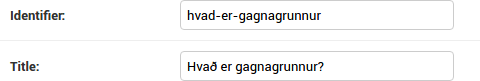
\includegraphics[width=0.7\textwidth]{identifier-selection}
\end{center}
\end{figure}


\chapter{Núverandi ástand og fyrirliggjandi betrumbætur} % Current status and future work
Sú vefsins sem fyrir liggur þegar þetta er skrifað er um ýmislegt megnugur. Tæknifær kennari eða kerfisstjóri getur sett upp keyrandi útgáfu af vefnum, sjá \myref{sec:installation}. Kennari eða annar efnishöfundur getur stofnað námskeið, samið greinar og æfingar og breytt þeim sem fyrir liggja. Nemandi getur skráð sig í námskeið, lesið greinar og fengið uppástungur um hvaða greinar mætti leysa næst, leyst verkefni sem fyrir viðkomandi eru sett og fengið afrek sín skrásett.

En að sjálfsögðu eru nokkur atriði þegar þekkt sem betur mættu fara \myref{sec:current-limitations} og önnur sem bæta má við\myref{sec:future-work}.
\section{Takmarkanir á núverandi útgáfu}
\label{sec:current-limitations}
\subsection{Greining á INSERT, UPDATE og DELETE skipunum}
Sem stendur eru \texttt{INSERT}, \texttt{UPDATE} og \texttt{DELETE} skipanir greindar með einföldum textasamanburði líkt og DDL-skipanir, sjá \myref{sec:other-command-analysis}.

Hægt væri að greina skipanirnar á hátt sem tekur tillit til virkni þeirra. Í öllum tilvikum væri um að ræða samanburð á mengi þeirra upplýsinga sem SQL-skipun nemandans skilur eftir sig og fyrirfram skilgreindu mengi.

Hins vegar er ekki sjálfgefið hvernig slíkur samanburður ætti að fara fram. Sérstaklega þyrfti að taka ákvörðun um hvaða hlutverk röðun gagnanna á að spila í samanburðinum. Þar til ástæða hefur fundist til að framkvæma samanburðinn á einn hátt frekar en annan er útfærsla á betri greiningu á þessum gerðum skipana í biðstöðu.
\subsection{Skrásetning}
\label{sec:logging}
Mögulegt er að skrásetja meiri upplýsingar um hvernig hver nemandi um sig notar vefinn. Sem stendur er einungis skráð hvaða æfingum nemendur ljúka sem og hvaða greinar hafa verið lesnar. Hægt væri að skrásetja til viðbótar hversu margar tilraunir voru gerðar við hvert verkefni og hversu löngum tíma var eytt í lestur á hverri grein. Þar fyrir utan væri mögulegt að útvíkka skrásetninguna enn frekar til að fá heildarmynd af notkun vefsins, sjá \myref{sec:flow}. Sömuleiðis mætti bæta tólin sem kennarar hafa yfir að ráða til að nálgast gögnin sem felast í notkun vefsins.
\subsection{Viðmótshönnun og útlit}
Útlit vefsins er tiltölulega einfalt, sjálfgefnar útlitsstillingar eru áberandi. Þetta kemur fram bæði í þeim hlutum vefsins sem snúa að nemendum og þeim hlutum sem snúa að efnishöfundum, þó með mismunandi hætti sé. 

Sá hluti vefsins sem snýr að nemendum notar Tufte CSS \myref{sec:tufte-css} til útfærslu. Lítið er brugðið út frá sjálfgefnum stillingum pakkans. Þá lita- og myndadýrð sem venjulega má finna á vefsíðum 2. áratugarins er ekki til staðar. Þetta veldur áhyggjum af því að litið verði á vefinn sem frumstæðan eða gamaldags.

Vandamál þeirra hluta sem snúa að kennurum og efnishöfundum eru af öðrum toga. Þar er viðmótið einfaldlega Django-ofurnotendaviðmót \myref{sec:django} sem hefur verið sérsniðið. Þó það sé ágætt til síns brúks og veiti mikinn aðgang að öllum nauðsynlegum gögnum, þá markast skipulag og innri forgangsröðun þess af tæknilegri útfærslu vefsins.

Fyrirkomulagið hefur sína kosti. Þar sem vefurinn er einfaldur hleðst hann hratt og afar ólíklegt er að efnishöfundar reki sig á illfyrirsjáanlegar takmarkanir á birtingarmöguleikum. En þó báðir hlutar vefsins séu fullkomlega nothæfir er ljóst að vefurinn sem heild myndi batna með aðkomu viðmótshönnuðar.
\section{Fyrirliggjandi verk}
\label{sec:future-work}
Auk þeirra atriða sem má bæta eru nokkur sem er borðliggjandi að bæta við.
\subsection{Leikjun}
\subsection{Flæðigreining}
\label{sec:flow}
Þar sem tengsl viðfangsefnanna eru sett fram sem net er auðvelt að sjá fyrir sér að upplýsingar felist í því hvernig nemendur ferðast þeirra á milli. Líta mætti á ferð nemenda um greinarnar sem flæði í neti, sem mætti greina.

Hægt væri að athuga algengustu vegi í gegnum netin, hvaða hnútar fá litla athygli og í hvaða hnútum sé algengt að fólk hætti lestrinum. Þessar upplýsingar gætu nýst við skipulag kennslu - sem og við endurbætur á skipulagi sjálfs vefsins.
\subsection{Hreyfing á myndum}
Blankenship og Dansereau\cite{blankenship2000effect} sýna að hreyfimyndir af netum geti haft kosti umfram kyrrstæðar myndir þegar kemur að getu nemenda til að muna upplýsingarnar sem í netinu fólust.

Efnisyfirlitsmyndir vefsins eru hreyfimyndir af netum. Í núverandi útgáfu er hreyfingin eingöngu notuð til að draga athygli að myndunum, en tæknilegu undirstöðurnar sem þyrfti til að stýra hreyfingunum nánar eru til staðar. Áhugavert væri að nýta markvisst forritaðar hreyfimyndir til að kynna uppbyggingu námsefnisins fyrir nemendum.

\bibliographystyle{plain}
\bibliography{master}

\appendix
\renewcommand{\chaptername}{Appendix}
\chapter{Kóðadæmi}
Hér má finna þann hluta grunnkóðans sem nefndur hefur verið í textanum. Allan grunnkóða má einnig finna á Github-síðu höfundar\footnote{\url{https://github.com/Ernir/sql-web}}.
\section{Django model klasar}
\label{code:django-model-objects}
\inputminted[fontsize=\scriptsize, frame=lines, linenos=true, python3=true, label=models.py]{python}{../sql\string_web/models.py}
\section{Keyrsluklasi æfinga}
\label{code:example-runner}
\inputminted[fontsize=\scriptsize, frame=lines, linenos=true, python3=true, label=sql_runner.py]{python}{../sql\string_web/sql\string_runner.py}
\section{Skilgreining Markdown-viðbótar}
\label{code:footnote-extension}
\inputminted[fontsize=\scriptsize, frame=lines, linenos=true, python3=true, label=footnotes.py]{python}{../sql\string_web/markdown\string_extensions/footnotes.py}
\section{Grunnskrá útlits}
\label{code:base-template}
\inputminted[fontsize=\scriptsize, frame=lines, linenos=true, label=base.html]{django}{../templates/base.html}

\chapter{Leyfi}
\label{sec:license}
Eftirfarandi opin leyfi eiga við forritskóða verkefnisins annars vegar og texta þess hins vegar.
\section{Forritskóði}\label{code}

This project's \emph{source code} is available under the MIT license, as
follows:

The MIT License (MIT)

Copyright (c) 2015-2017 Eiríkur Ernir Þorsteinsson

Permission is hereby granted, free of charge, to any person obtaining a
copy of this software and associated documentation files (the
``Software''), to deal in the Software without restriction, including
without limitation the rights to use, copy, modify, merge, publish,
distribute, sublicense, and/or sell copies of the Software, and to
permit persons to whom the Software is furnished to do so, subject to
the following conditions:

The above copyright notice and this permission notice shall be included
in all copies or substantial portions of the Software.

THE SOFTWARE IS PROVIDED ``AS IS'', WITHOUT WARRANTY OF ANY KIND,
EXPRESS OR IMPLIED, INCLUDING BUT NOT LIMITED TO THE WARRANTIES OF
MERCHANTABILITY, FITNESS FOR A PARTICULAR PURPOSE AND NONINFRINGEMENT.
IN NO EVENT SHALL THE AUTHORS OR COPYRIGHT HOLDERS BE LIABLE FOR ANY
CLAIM, DAMAGES OR OTHER LIABILITY, WHETHER IN AN ACTION OF CONTRACT,
TORT OR OTHERWISE, ARISING FROM, OUT OF OR IN CONNECTION WITH THE
SOFTWARE OR THE USE OR OTHER DEALINGS IN THE SOFTWARE.

\section{Texti}\label{contents}

This project's textual contents are modifiable under Creative Commons,
\href{http://creativecommons.org/licenses/by-nc-sa/4.0/}{CC BY-NC-SA
4.0}.

\chapter{Uppsetningarleiðbeiningar}
\label{sec:installation}
Nýjustu útgáfu uppsetningarleiðbeininga má finna á Github-síðu höfundar\footnote{\url{https://github.com/Ernir/sql-web/blob/master/README.md}}. Þær eru endurteknar hér að neðan.

\section*{SQLweb}\label{sqlweb}

\textbf{(Ísl)} Kennsluvefur í notkun gagnasafna. Hluti af
meistaraverkefni Eiríks Ernis Þorsteinssonar við IVT-deild Háskóla
Íslands. Uppsetningarleiðbeiningar má finna að neðan.

\textbf{(En)} A teaching website for introductory database usage.
Written as a part of Eiríkur Ernir Þorsteinsson's master's project,
Faculty of Industrial Engineering, Mechanical Engineering, and Computer
Science at the University of Iceland. Installation instructions are
currently in Icelandic only, but can be found below.

\subsection*{Uppsetning
þróunarútgáfu}\label{uppsetning-uxferuxf3unaruxfatguxe1fu}

Vefurinn er skrifaður í \href{https://www.djangoproject.com/}{Django} og
ætti að keyranlegur á flestum nútíma stýrikerfum. Þessar
uppsetningarleiðbeiningar gera ráð fyrir
\href{https://www.ubuntu.com/}{Ubuntu} Linux 16.04 eða sambærilegu
kerfi. Gert er ráð fyrir að lesandinn sé kunnugur skipanalínunotkun.

\subsubsection{0. Undanfarar}\label{undanfarar}

Áður en hafist er handa er nauðsynlegt að eftirfarandi sé uppsett:

\begin{itemize}
\item
  \href{https://www.python.org/downloads/}{python 3} með þróunartólum,
  sýndarumhverfakerfi og pakkakerfi (nauðsynlegt)
\item
  þýðingartól sem tengjast C- og Postgresviðbótum
\item
  gagnagrunnskerfi, hér gert ráð fyrir
  \href{https://sqlite.org/}{SQLite}
\end{itemize}

að auki er sterklega mælt með: * \href{https://git-scm.com/}{git} til að
sækja og viðhalda forritskóða * cURL og tar til að sækja myndir

Á Ubuntu má setja þetta allt saman upp með eftirfarandi skipunum:

\begin{minted}[fontsize=\small, frame=lines]{bash}
$ sudo apt-get update && sudo apt-get upgrade
$ sudo apt-get install git python3-dev python3-pip 
    python3-venv sqlite3 build-essential libpq-dev curl
\end{minted}

\subsubsection{1. Stilling á
umhverfisbreytum}\label{stilling-uxe1-umhverfisbreytum}

Keyrsla vefsins krefst þess að tvær umhverfisbreytur (e.
\emph{environment variables}) séu stilltar. Þær eru
\texttt{DEBUG\_MODE}, sem við þróun ætti að vera \texttt{1} og
\texttt{SECRET\_KEY} sem er ekki-tómur strengur.

Á staðaluppsettu Ubuntu er að afgreiða breyturnar með því að setja línur
á borð við eftirfarandi í \texttt{.bashrc} skrána og endurhlaða svo
breytunum (t.d. með því að endurræsa skelina).

\begin{minted}[fontsize=\small, frame=lines]{bash}
export SECRET_KEY="lykill"
export DEBUG_MODE="1"
\end{minted}

Í raunverulegu keyrsluumhverfi ætti \texttt{SECRET\_KEY} að vera langur
strengur sem erfitt er að giska á og \texttt{DEBUG\_MODE} að vera 0.

\subsubsection{2. Forritskóði sóttur}\label{forritskuxf3uxf0i-suxf3ttur}

Til að ná í nýjustu útgáfu af forritskóða vefsins má nota git. Færum
okkur í yfirmöppu þeirrar möppu sem vefurinn skal dvelja í og sækjum
þvínæst forritskóðann með:

\begin{minted}[fontsize=\small, frame=lines]{bash}
$ git clone https://github.com/Ernir/sql-web.git
\end{minted}

en skipunin mun búa til möppu að nafni \texttt{sql-web}. Færum okkur til
hennar og höldum okkur þar þangað til uppsetningu er lokið.

\begin{minted}[fontsize=\small, frame=lines]{bash}
$ cd sql-web/
\end{minted}

\emph{Annar valmöguleiki}: Hægt er að sækja forritskóðann án þess að
nota git með því að fara inn á
\href{https://github.com/Ernir/sql-web}{github-síðu verkefnisins} og
sækja hana sem .zip skrá.

\subsubsection{3. Uppsetning og virkjun
sýndarumhverfis}\label{uppsetning-og-virkjun-suxfdndarumhverfis}

Ráðlagt er að keyra Python-forrit önnur en hin fánýtustu í
sýndarumhverfi (e. \emph{virtual environment}) sem heldur utan um
forritssöfn. Stofnum til nýs sýndarumhverfis að nafni \texttt{sqlvenv}.

\begin{minted}[fontsize=\small, frame=lines]{bash}
$ python3 -m venv sqlvenv
\end{minted}

Áður en umhverfið má nota þarf að virkja það. Að óbreyttu mun nafn
sýndarumhverfisins birtast fremst á skipanalínunni meðan það er virkt.

\begin{minted}[fontsize=\small, frame=lines]{bash}
$ source sqlvenv/bin/activate
(sqlvenv) $ 
\end{minted}

\emph{Athugasemd}: Ekki er þörf á því núna, en til að slökkva á
sýndarumhverfinu má gefa skipunina \texttt{deactivate}.

\begin{minted}[fontsize=\small, frame=lines]{bash}
(sqlvenv) $ deactivate 
$
\end{minted}

\subsubsection{4. Uppsetning pakka sem vefurinn
krefst}\label{uppsetning-pakka-sem-vefurinn-krefst}

Í möppunni \texttt{sql-web} má finna skrá sem heitir
\texttt{requirements.txt}, sem inniheldur upplýsingar um forritssöfn sem
vefnum eru nauðsynleg. Setjum söfnin upp með \texttt{pip}
pakkastjórnunarkerfinu.

Í þessu skrefi er mikilvægt að sýndarumhverfið sé virkt!

\begin{minted}[fontsize=\small, frame=lines]{bash}
(sqlvenv) $ pip install -r requirements.txt
\end{minted}

\subsubsection{5. Uppsetning gagna
(valkvæmt)}\label{uppsetning-gagna-valkvuxe6mt}

Með forritskóðanum fylgja sjálfgefin gögn - þ.e.a.s. innihald
kennslubókarinnar sjálfrar ásamt sýnidæma um verkefni. Til að setja
gögnin upp þarf að keyra tvær skipanir, sú fyrri til að setja upp
gagnagrunn og þá seinni til að hlaða í hann gögnum.

\begin{minted}[fontsize=\small, frame=lines]{bash}
(sqlvenv) $ python manage.py migrate
(sqlvenv) $ python manage.py loaddata content.json
\end{minted}

Sjálfgefnu gögnin innihalda vísanir í myndir. Myndirnar eiga heima í
skrá sem heitir \texttt{mediafiles} og er undirmappa \texttt{sql-web}
möppunnar. Eftirfarandi skipun (sem krefst cURL og tar) sækir myndirnar
og setur þær í viðeigandi möppu:

\begin{minted}[fontsize=\small, frame=lines]{bash}
(sqlvenv) $ curl https://notendur.hi.is/~ernir/sql-web/mediafiles.tar.gz | tar -xz
\end{minted}

\emph{Annar valmöguleiki}: Hægt er að komast hjá því að nota cURL og/eða
tar með því að búa til \texttt{mediafiles} möppuna handvirkt og sækja
myndirnar sem
\href{https://notendur.hi.is/~ernir/sql-web/mediafiles.zip}{.zip skrá}.
Þetta gæti verið viðeigandi fyrir Microsoft Windows notendur.

\subsubsection{6. Uppsetning ofurnotandareiknings
(valkvæmt)}\label{uppsetning-ofurnotandareiknings-valkvuxe6mt}

Setja þarf upp ofurnotanda fyrir vefinn ef gera á efnisbreytingar. Það
má gera með skipuninni

\begin{minted}[fontsize=\small, frame=lines]{bash}
(sqlvenv) $ python manage.py createsuperuser
\end{minted}

og fylgja leiðbeiningunum sem birtast á skjánum.

\subsubsection{7. Keyrsla
þróunarvefþjóns}\label{keyrsla-uxferuxf3unarvefuxfejuxf3ns}

Með Django fylgir vefþjónn sem er hentugur til keyrslu á þróunarvélum. Á
honum má kveikja með skipuninni

\begin{minted}[fontsize=\small, frame=lines]{bash}
(sqlvenv) $ python manage.py runserver
\end{minted}

og heimsækja svo síðuna með því að fara á slóðina
\texttt{http://127.0.0.1:8000/} í vafra.

Til að breyta eða bæta við námskeiðum, lesefni eða verkefnum má fara inn
á slóðina \texttt{http://127.0.0.1:8000/admin} og skrá sig inn með
ofurnotendaaðganginum sem búinn var til í skrefi 5.

\subsection*{Uppsetning
keyrsluútgáfu}\label{uppsetning-keyrsluuxfatguxe1fu}

Uppsetning keyrsluútgáfu (til opinberrar birtingar) er í flestum atriðum
eins og uppsetning þróunarútgáfu. Af öryggisástæðum þarf þó að gera
breytingar á umhverfisbreytum, sjá skref 1 í uppsetningu þróunarútgáfu.

\begin{minted}[fontsize=\small, frame=lines]{bash}
export SECRET_KEY="miklulengristrengurenþetta"
export DEBUG_MODE="0"
\end{minted}

Auk þess þarf að setja upp afkastameiri og öruggari vefþjón en þróunarvefþjóninn sem er innbyggður í Django.
Þekkt er að \href{http://gunicorn.org/}{Gunicorn} með \href{https://www.nginx.com/}{NGINX} hentar vel.
\end{document}